\documentclass{beamer}
\usetheme{Boadilla}
\usepackage{amsmath,amssymb,graphics}
\title{Estimation Techniques in Mixture of Regression Model}
\author{Subhrajyoty Roy (BS - 1613)}
\date{March 4, 2019}
\begin{document}
	\begin{frame}
		\titlepage
	\end{frame}
	\begin{frame}
		\frametitle{The Historical Example}
		Elizabeth Cohen, in 1980, wanted to study music perception of eastern and western musicians by an experiment conducted at Center for Research in Music and Acoustics (CRMA), Stanford University.
		\begin{enumerate}
			\item \textbf{Tuning Ratio:} The ratio of the harmonics to the fundamental tone (A major i.e. 440 cps). The harmonics is played to the musicians. It is chosen to be varied from 1.35 to 3.0
			\item \textbf{Response Ratio:} The ratio of harmonics to the fundamental tone that the musician tunes in his/her instrument.
		\end{enumerate}
	\end{frame}
\begin{frame}
	\begin{figure}
	\caption{Scatterplot of Cohen's experiment}
	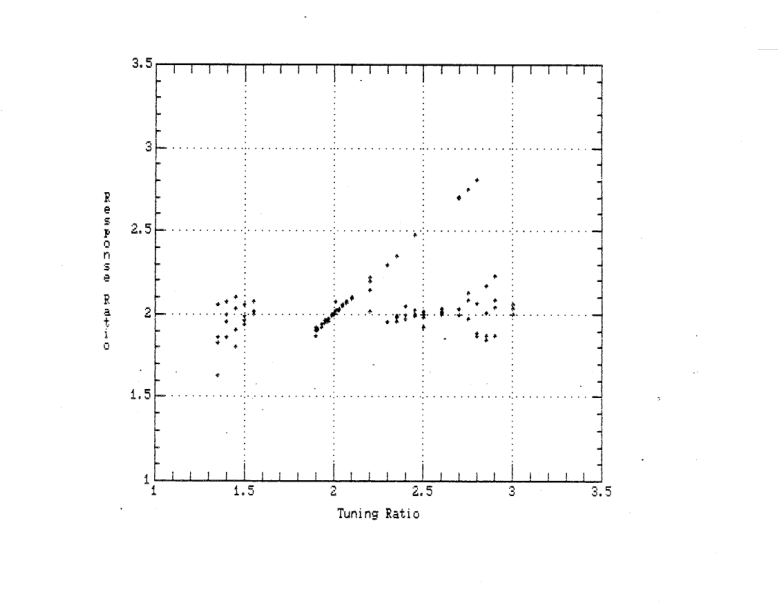
\includegraphics[width=\linewidth]{cohen.png}
	\end{figure}
\end{frame}
\begin{frame}
	\frametitle{The Mathematical Model}
	Cohen's experiment was not the first. The model existed long before in \textbf{Econometrics}, introduced by Richard Quandt and James Ramsey, under the name of switching regression.\\
	Let us consider the usual setup of regression where $y_i$'s are the responses and $x_i$'s are the predictor vectors with errors denoted by $\epsilon_i$'s. The regression coefficients are $\beta_j$ vector. Consider new parameters $\pi_j$'s for $j=1,2\dots k$, with $\sum_j \pi_j = 1$.
	$$y_i = \begin{cases}
		{x'}_i \beta_1 + \epsilon_{i1} & \text{w.p. } \pi_1\\
		{x'}_i \beta_2 + \epsilon_{i2} & \text{w.p. } \pi_2\\
		\dots & \dots \\
		{x'}_i \beta_k + \epsilon_{ik} & \text{w.p. } \pi_k\\
	\end{cases}$$
	where $\epsilon_{ij} \sim N(0, \sigma_j^2)$ and these are independent.\\
	The free parameters are $\theta = \left( \beta_1, \dots \beta_k, \sigma_1^2, \dots, \sigma_k^2, \pi_1,\dots \pi_{k-1} \right)$
\end{frame}
\begin{frame}
	\frametitle{Why it has not been studied before?}
	\textbf{MOM:} Karl Pearson tried to estimate parameters of 2 sized mixture of Normal distributions $f(x) = \lambda N(\mu_1, \sigma_1^2) + (1-\lambda) N(\mu_2, \sigma_2^2)$ using method of moments technique in 1894. Equate first five population and sample central moments, and after some \textbf{messy} algebra, he showed that it requires the solution for the equation;
	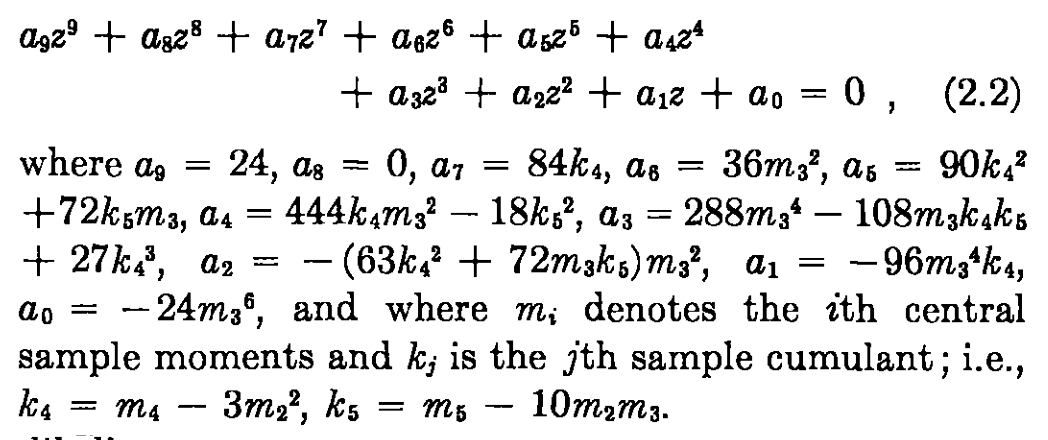
\includegraphics[width = 0.8\linewidth]{./nonic.png}\\
	\textit{Nobody ever dared to do the same for Regression Mixture!}
\end{frame}

\begin{frame}
\frametitle{Why it has not been studied before? (Contd.)}
\small 
\textbf{MLE:} Consider the case with only $k=2$. 
\begin{align*}
	\mathcal{L}(\lambda,\beta,\sigma) & = \prod_{i=1}^{n}\left[ \sum_{j=1}^2 \lambda_j (2\pi \sigma_j^2)^{-1/2} \exp\left\{ -\frac{1}{2\sigma_j^2} (y_i - x'_i\beta_j)^2 \right\} \right]\\
	& \geq \prod_{i=1}^{n}\left[ \sum_{j=1}^2 (8\pi \sigma_j^2)^{-1/2} \exp\left\{ -\frac{1}{2\sigma_j^2} (y_i - x'_i\beta_j)^2 \right\} \right]\\
	& = \prod_{i=2}^{n}\left[ \sum_{j=1}^2 (8\pi \sigma_j^2)^{-1/2} \exp\left\{ -\frac{1}{2\sigma_j^2} (y_i - x'_i\beta_j)^2 \right\} \right]\\
	& \times \frac{1}{2\sqrt{2\pi}}\sum_{j=1}^2 \frac{1}{\sigma_j}\exp\left\{ -\frac{1}{2\sigma_j^2} (y_1 - x'_1\beta_j)^2 \right\}\\
	& \geq \prod_{i=2}^{n} \frac{1}{2\sqrt{2\pi}\sigma_2}\exp\left\{ -\frac{1}{2\sigma_2^2} (y_i - x'_i\beta_2)^2 \right\} \times \frac{1}{2\sqrt{2\pi}\sigma_1}
\end{align*}
Day (1969) stated that \textit{"Maximum likelihood clearly breaks down!"}\\
\end{frame}

\begin{frame}
	\frametitle{What is the way out then?}
	Even if both MOM and MLE approach does not show promises;
	\begin{enumerate}
		\item W.Y. Tan and W.C.Chang (1972) in economics.
		\item Fryer J.G. and Robertson C.A (1972) in biological sciences.
		\item Hosmer D. W. (1973) in biology.
		\item Hosmer D.W. (1974) in communication science.
	\end{enumerate}
	reported "good" estimates using iterative techniques based on maximum likelihood approach. However, everyone concluded that the choice of initial values is crucial.\\
	Kiefer (1978), showed that MLE techniques have some hope.\\
	De Veaux (1986 \& 1989) thinks of using EM Algorithm in the problem. 
\end{frame}


\begin{frame}
	\frametitle{Consistency of solution of Likelihood Equation}
	\begin{theorem}
		Let $f(z;\theta)$ be density, with unknown parameter vector $\theta$ residing in a closed parameter space $\Omega$. $z_1, z_2, \dots z_n$ are i.i.d. observations. Let $\theta_0$ be true parameter value. Under some \textbf{regularity conditions}, there exists $\theta_n$, solution of the log-likelihood equation;
		$$\frac{\partial\log\mathcal{L}}{\partial\theta} = 0$$
		such that $\sqrt{n}(\theta_n - \theta_0) \rightarrow N(0, I(\theta_0)^{-1})$.
	\end{theorem}
	The univariate version is proved by Harald Cramer, and the multivariate version is done by Tarone and Gruenhage.
\end{frame}
\begin{frame}
	\frametitle{The regularity conditions}
	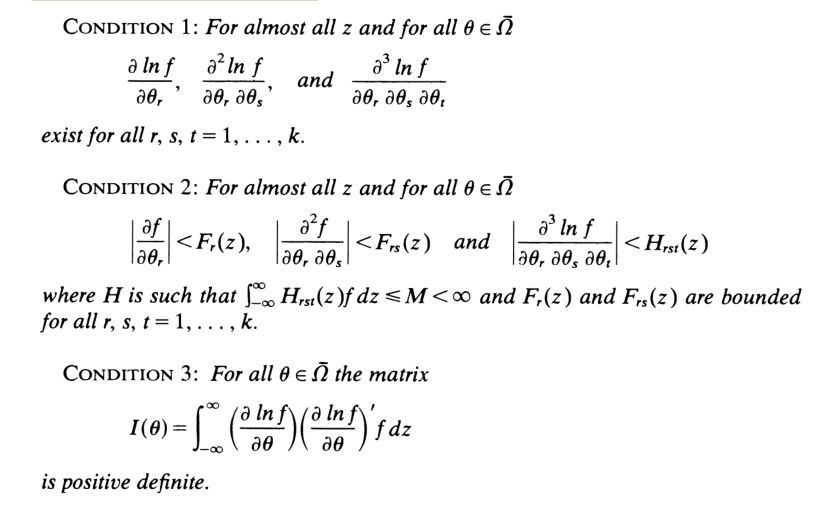
\includegraphics[width = \linewidth]{./reg_conditions.png}
\end{frame}

\begin{frame}
	\frametitle{Kiefer's Conclusion}
	\begin{itemize}
		\item Consider a closed region $\Omega$ containing the true parameter value $\theta_0$ for mixture of regression setup, which does not contain the boundary cases $\lambda = 0, \lambda = 1, \sigma_1 = 0$ and $\sigma_2 = 0$, then the mixture density satisfies the regularity conditions.
		\item Kiefer verified this by simply differentiating the log likelihood.
		\item He noted that $I(\theta)$ is not positive definite if and only if $y_i/x_i$ is a fixed constant for any $i=1,2,\dots n$.
		\item Kiefer also noted that the above theorem does not show whether there are multiple consistent estimators, also how to find them. He exclaimed we can simply use Newton-Raphson method to find the solution of log likelihood equation.
		\item Quandt and Ramsey performed some simulation exercises using Newton Raphson method, and found the root to heavily depend on the initial value. They suspected the likelihood has numerous local maxima, and only a few of them are actually consistent.
	\end{itemize}
\end{frame}

\begin{frame}
	\frametitle{A basic EM Algorithm}
	As soon as EM Algorithm emerges, people found that Mixture of Regression can be iteratively solved using EM Algorithm.
	\begin{itemize}
		\item ${\ell}(\theta) = \sum_{i=1}^{n} \log \left( \sum_{j=1}^{k} \pi_j\phi_j(y_i\vert x_i) \right)$ where $\phi_j(\cdot\vert x_i)$ is normal density with mean $x'_i\beta_j$ and variance $\sigma_j^2$.
		\item Think of the complete data by introducing the latent variable $w_{ij}$, denoting the indicator whether $y_i$ comes from component $j$.
		\item Given $\theta^{(t)}$, expected "complete" log-likelihood is;
		$$Q(\theta; \theta^{(t)}) = \sum_{i=1}^{n} \left( \sum_{j=1}^{k} - w_{ij}^{(t)} \left(\frac{y_i - x'_i\beta_j}{\sigma_j}\right)^2 \right) + \dots $$
		where $w_{ij}^{(t)} = \frac{\pi_j^{(t)}\phi_j(y_i\vert x_i)}{\sum_{j=1}^{k} \pi_j^{(t)}\phi_j(y_i\vert x_i)}$.
	\end{itemize}
\end{frame}

\begin{frame}
	\begin{itemize}
		\item Maximizing $Q(\theta; \theta^{(t)})$ with respect to $\beta_j$ is same as performing a weighted regression exercise, of $y_1, y_2, \dots y_n$ on $x_1, x_2, \dots x_n$ with weights $w_{1j}, w_{2j}, \dots w_{nj}$.
		\item The updation rule hence is;
		\begin{align*}
			\beta_j^{(t+1)} & = \left( X'W_jX \right)^{-1} X'W_jy\\
			\sigma_j^{2(t+1)} & = \frac{\sum_{i=1}^{n} w_{ij}^{(t)} (y_i - x'_i\beta_j^{(t+1)})^2}{\sum_{i=1}^{n} w_{ij}^{(t)}}\\
			\pi_j^{(t+1)} & = \frac{\sum_{i=1}^{n} w_{ij}^{(t)}}{n}
		\end{align*}
		where $W_j$ is the diagonal matrix with elements $w_{1j}, w_{2j}, \dots w_{nj}$.
	\end{itemize}
\end{frame}

\begin{frame}
	\frametitle{Other types of EM: ECM}
	\begin{itemize}
		\item At the end of E step, we have $w_{ij}^{(t)}$.
		\item C-step classifies the sample points to the components. Create a partition $P^{(t+1)} = \left\{ P_1^{(t+1)}, P_2^{(t+1)}, \dots P_k^{(t+1)} \right\}$, where
		$$P_j^{(t+1)} = \left\{ (x_i, y_i) : j = \arg_h\max w_{ih}^{(t)} \right\}$$
		\item The M-step is exactly same as before, with the same $w_{ij}^{(t)}$'s.
		\item \textbf{Q: Why bother doing C-step?}\\
		Allows dynamic number of components. If any of $P_j^{(t+1)}$ is empty or \textit{has only one observation}, restart with $(k-1)$ components.
		  
	\end{itemize}
\end{frame}


\begin{frame}
	\frametitle{Other types of EM: ESM}
	\begin{itemize}
		\item Same E-step as basic EM.
		\item Rather than classifying the observation to components based on highest posteriors, simulate the classification according to multinomial distribution. Therefore,
		$$P_j^{(t+1)} = \left\{ (x_i, y_i) : e_j \sim Multinomial(1, w_{i1}, w_{i2}, \dots w_{ik}) \right\}$$
		where $e_j$ is the vector of size $k$ with 1 at position $j$ and 0 at other places.
		\item The M-step is same as in basic EM.
		\item Allows dynamic component numbers, but is not too rigid about classifying.
		\item Emperically performs better when the initial estimates are random.
	\end{itemize}
\end{frame}

\begin{frame}
	\frametitle{Is EM a good thing to do?}
	\begin{theorem}[De Veaux, 1986]
		Let $x_i, y_i, i=1,2,\dots n$ be independent samples from mixture of regression problem. Let $\hat{\theta}_n$ be a $\sqrt{n}$-consistent estimator of $\theta = (\lambda, \alpha_1, \alpha_2,\beta_1,\beta_2,\sigma_1^2, \sigma_2^2)$. Let $\left\{ \theta^{(t)} \right\}_{t\geq 0}$ be the EM algorithm sequence starting at $\hat{\theta}_n$. Then, $\theta_n^* = \lim_{t\rightarrow 0}\theta^{(t)}$ is asymptotically efficient for estimating $\theta$.
	\end{theorem}
\end{frame}

\begin{frame}
	\frametitle{Some important results of EM Algorithm}
	\begin{theorem}[Dempster, Laird, Rubin 1977]
		EM Algorithm never decreases the log-likelihood.
		$$\ell(\theta^{(t+1)}) \geq \ell(\theta^{(t)})$$.
	\end{theorem}
	
	\begin{theorem}[Wu, 1983]
		If both "complete" and "incomplete" likelihoods are continuously differentiable w.r.t. $\theta$ and the parameter space $\theta$ is a compact subset of $\mathbb{R}^*$, then any sequence of $\theta^{(t)}$  produced by EM Algorithm converges to some stationary point $\theta^*$ of the log-likelihood.
	\end{theorem}
\end{frame}

\begin{frame}
	\frametitle{De Veaux's Result on Convergence of EM Algorithm}
	\begin{theorem}[De Veaux, 1986]
		Let $x_i, y_i, i=1,2,\dots n$ be independent samples from mixture of regression problem. Let $\hat{\theta}_n$ be a $\sqrt{n}$-consistent estimator of $\theta = (\lambda, \alpha_1, \alpha_2,\beta_1,\beta_2,\sigma_1^2, \sigma_2^2)$. Let $\left\{ \theta^{(t)} \right\}_{t\geq 0}$ be the EM algorithm sequence starting at $\hat{\theta}_n$. Then, $\theta_n^* = \lim_{t\rightarrow 0}\theta^{(t)}$ is asymptotically efficient for estimating $\theta$.
	\end{theorem}

	\textbf{Note:} The proof do not require the initial estimates to be actually $\sqrt{n}$-consistent. $\hat{\theta}_n$ should be "close" so that we have a convex log-likelihood there.
\end{frame}

\begin{frame}
	\frametitle{Good MM estimates to start with}
	\begin{enumerate}
		\item Choose three non-overlapping bins $I_1, I_2, I_3$ on x-axis.
		\item Assume each bin contains same number of points. (!important)
		\item Obtain estimates for each bin $(\hat{\lambda}, \hat{\mu}_1, \hat{\mu}_2, \hat{\sigma}_1, \hat{\sigma}_2)$ as $(0.5, \bar{y}- s/2, \bar{y} + s/2, s/2, s/2)$. Assume, $\hat{\mu}_1 < \hat{\mu}_2$.
		\item Obtain the pair of straight lines, the straight pair $(\hat{\alpha}_{1s}, \hat{\alpha}_{2s}, \hat{\beta}_{1s}, \hat{\beta}_{2s})$ and the crossed pair $(\hat{\alpha}_{1c}, \hat{\alpha}_{2c}, \hat{\beta}_{1c}, \hat{\beta}_{2c})$.
		\item Calculate total distances from pair of regression lines to the points $(\bar{x}_3, \hat{\mu}_1^{(3)})$ and $(\bar{x}_3, \hat{\mu}_2^{(3)})$.
		\item Choose the minimizing one as initial estimates for beta coefficients.
	\end{enumerate}
\end{frame}

\begin{frame}
	\frametitle{Binning Algorithm in Action (Step 1)}
	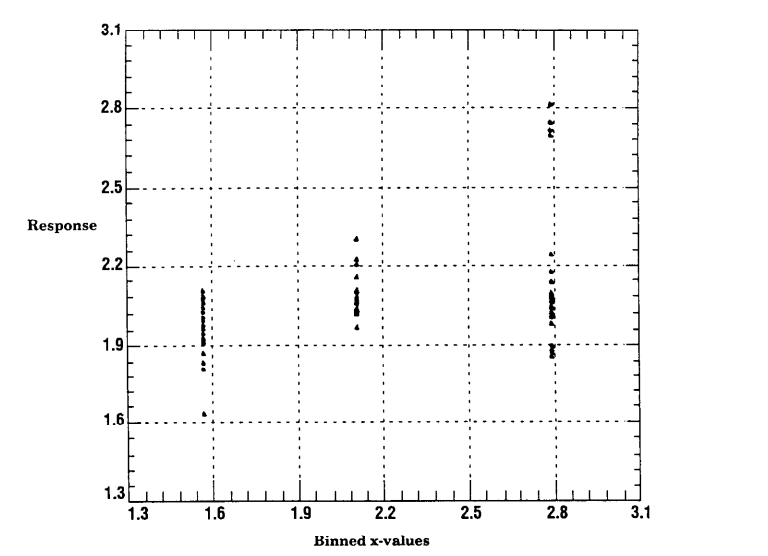
\includegraphics[height = 3in]{./mm_1.png}
\end{frame}

\begin{frame}
	\frametitle{Binning Algorithm in Action (Step 2)}
	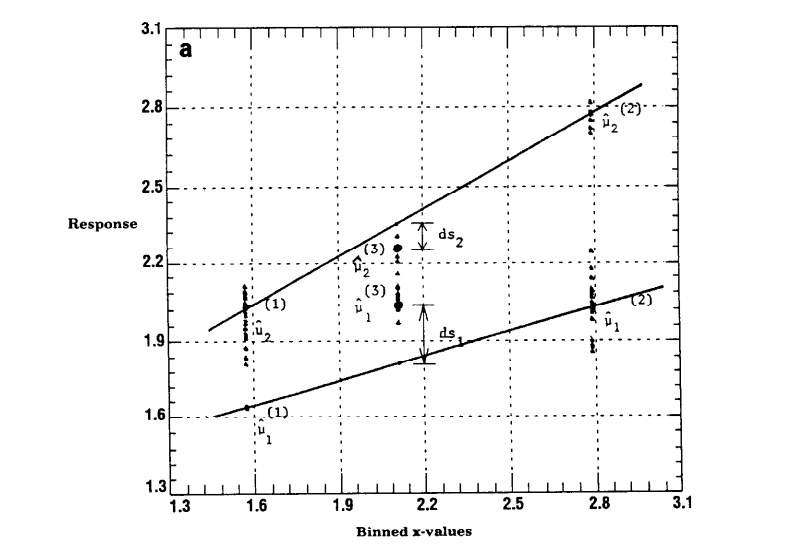
\includegraphics[height = 3in]{./mm_2.png}
\end{frame}

\begin{frame}
	\frametitle{Binning Algorithm in Action (Step 3)}
	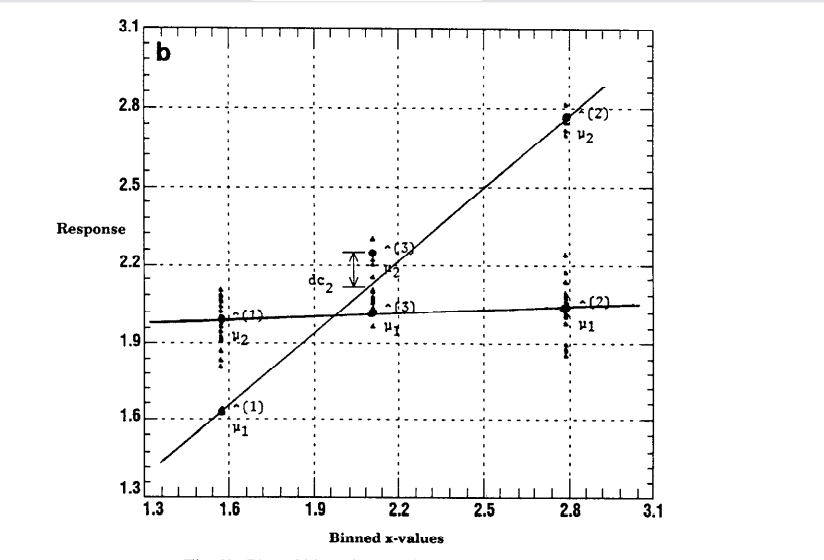
\includegraphics[height = 3in]{./mm_3.png}
\end{frame}


\begin{frame}
	\frametitle{Does this binning Algorithm gives a "good" starting point?}
	\textbf{No}, in the way we described it.\par 
	\textbf{Yes}, if the estimates for each interval is $\sqrt{m}$-consistent, where $m$ is the number of datapoints in each bin.\\
	\begin{itemize}
		\item Later, it has been proved that if $\lambda_0 = 0.5$ (Jones \& MchLachlan, 1992 and Turner, 2000), then the binning procedure gives $\sqrt{n}$-consistent starting point for EM.
		\item Current Algorithms implemented in different software packages, tries with random values of $\lambda$ as starting point, and performs the estimation several times.
		\item Standard errors of the estimates are obtained using Bootstrapping.
	\end{itemize}
\end{frame}

\begin{frame}
	\frametitle{Some Simulations}
	A dataframe was generated with a single predictor $x$ and the response $y$ modeled as;
	$$y = \begin{cases}
		-4 + 3x + \epsilon & \text{for class 1}\\
		12 - 2x + \epsilon & \text{for class 2}
	\end{cases}$$
	where $\epsilon \sim N(0,9)$.
	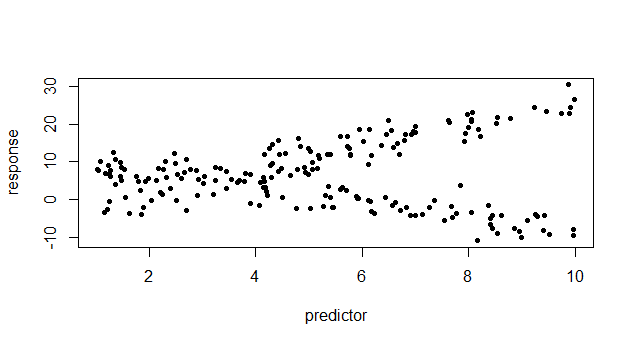
\includegraphics[width=\linewidth]{./simplot_1.png}
\end{frame}

\begin{frame}
	\frametitle{Some Simulations (Contd.)}
	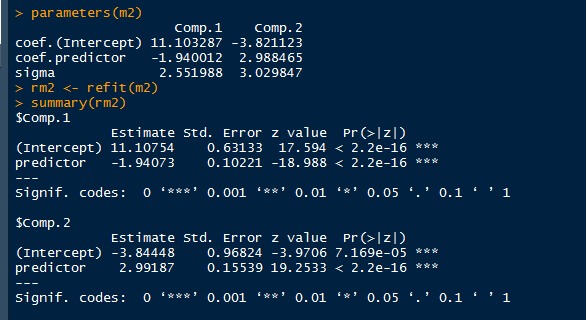
\includegraphics[width = \linewidth]{./sim_results.png}
\end{frame}

\begin{frame}
	\frametitle{Some Simulations (Contd.)}
	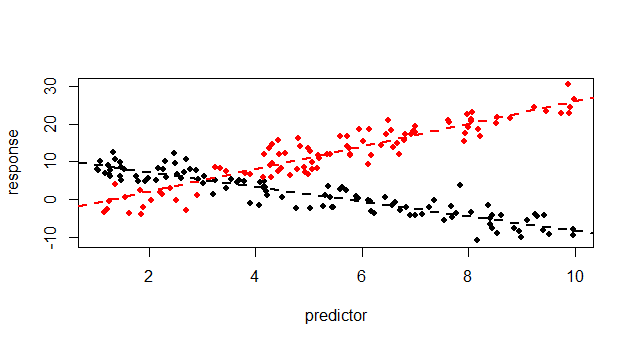
\includegraphics[width = \linewidth, height = 3in]{./simplot_2.png}
\end{frame}

\begin{frame}
	\frametitle{A Practical Example: Predicting Sold Status of Tea Lots}
	\begin{figure}
		\caption{Predicted Probabilities vs Actual Probabilities for Logistic Regression}
		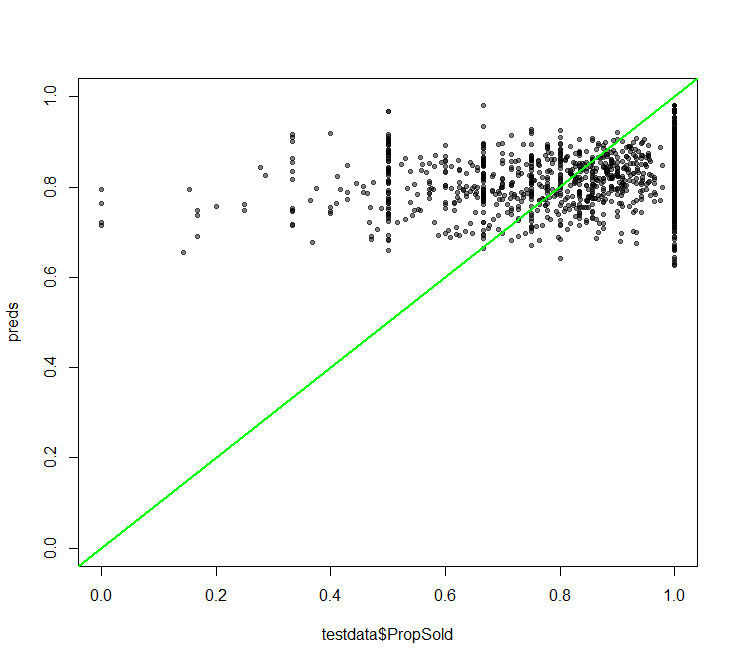
\includegraphics[height= 2.7in]{./pracplot_1.png}
	\end{figure}
\end{frame}

\begin{frame}
\frametitle{A Practical Example: Predicting Sold Status of Tea Lots}
\begin{figure}
	\caption{Predicted Probabilities vs Actual Probabilities for GAM}
	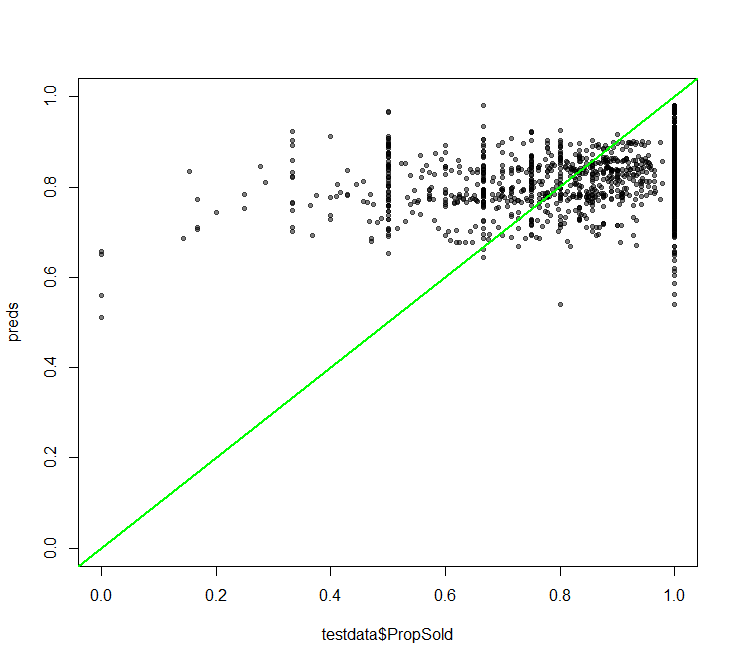
\includegraphics[height= 2.7in]{./pracplot_2.png}
\end{figure}
\end{frame}

\begin{frame}
\frametitle{A Practical Example: Predicting Sold Status of Tea Lots}
\begin{figure}
	\caption{Predicted Probabilities vs Actual Probabilities for 3 component Mixture of Logistic Regression}
	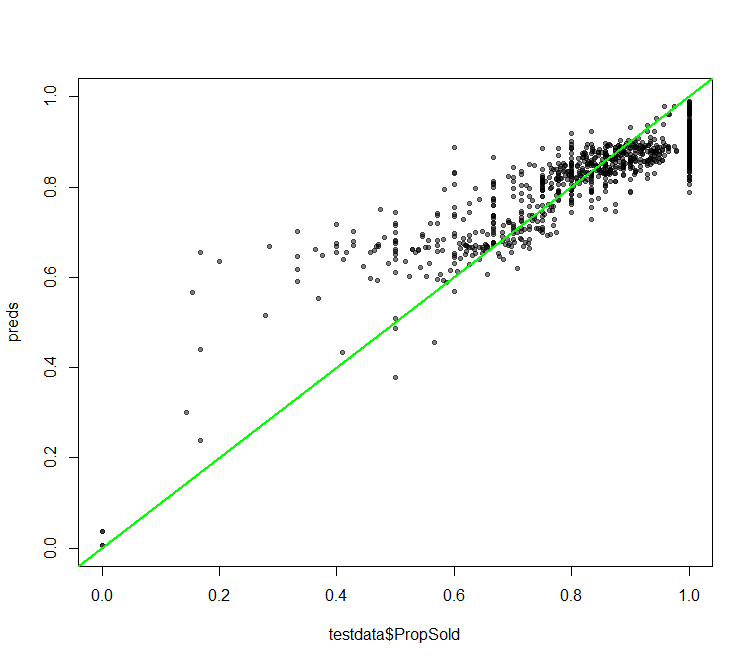
\includegraphics[height= 2.7in]{./pracplot_3.png}
\end{figure}
\end{frame}


\begin{frame}
	\frametitle{References}
	\begin{enumerate}
		\item \textit{Mixtures of Linear Regression}, Richard De Veaux (1989) Computational Statistics \& Data Analysis Vol - 8, pp 227-245.
		\item \textit{Parameter Estimation for a mixture of Linear Regressions}, Richard De Veaux, Technical Report 247, April 1986, Dept. of Statistics, Stanford University.
		\item \textit{Fitting mixtures of linear regressions}, Susana Faria \& Gilda Soromenho, Journal of Statistical Computation and Simulation Vol.80, no. 2, February 2010, pp 201-225.
		\item \textit{Discrete Parameter Variation: Efficient Estimation of a Switching Regression Model}, Nicholas M. Kiefer, Econometrica, Vol. 46, No. 2, March 1978, pp 427-434.
		\item \textit{Estimating Mixtures of Normal Distributions and
			Switching Regressions}, Richard E. Quandt \& James B. Ramsey (1978), Journal of American Statistical Association, 73:364, pp 730-738.
	\end{enumerate}
\end{frame}


\begin{frame}
	\begin{center}
		\Huge 
		\textit{THANK YOU}
	\end{center}
\end{frame}

\end{document}












